\documentclass[dvipdfmx]{beamer}
\usepackage{pxjahyper}
%\usetheme{Frankfurt}%Frankfurt,AnnArbor, Antibes, Berlin, Berkeley, Bergen, Boadilla, boxes, Copenhagen

%\beamerdefaultoverlayspecification{<+->}% 箇条書きを段階的にみせたいとき
%\setbeamercovered{transparent}%隠してるアイテムを半透明で表示
\renewcommand{\kanjifamilydefault}{\gtdefault}%日本語フォントをゴシックに
\usepackage{graphicx}% 各種画像の張り込み

%\usepackage[english]{babel}%多言語文書を作成する
\usepackage{amsmath,amssymb}%標準数式表現を拡大する
\setbeamertemplate{footline}[frame number] 

%---------- テーマの設定 ----------%
\usetheme{Madrid} %テーマ
\usecolortheme[named=orange]{structure} %テーマの色


%---------- テーマの設定 ----------%

%ここからスライド内容

%表紙
\title{\bfseries ゼミ発表}
%\subtitle{サブタイトル}


\author{学籍番号:16344217 \\氏名:津上祐典}
\institute[]{九州工業大学大学院 工学府\\機械知能工学専攻 知能制御工学コー
ス 西田研究室}

\date{2016年6月23日}
\subject{\LaTeX{}+Beamer}

%タイトルの表示
\begin{document}
\begin{frame}
 \titlepage 
\end{frame}

%目次の設定
\begin{frame}<beamer> 
  \frametitle{目次}
  \tableofcontents
\end{frame}

\section{研究背景} %目次に表示するスライド名
\begin{frame}{研究背景} %スライドのタイトル
 \begin{itemize}
  \item グリッパの自動交換
  \item 複雑な把持計画
  \item これらの作業は\alert{ボトルネック}
 \end{itemize}
\end{frame} 

\section{MR$\alpha$流体グリッパ}

\subsection{原理}



\begin{frame}{原理}
\begin{block}{ラベル} 
内容
\end{block}
\begin{block}{ER流体}
電界で変化
\end{block}

\pause %アニメーション:後から表示する
\begin{alertblock}{結果}
MR流体のほうがいいね
\end{alertblock}
\end{frame}



\section{写真}

\subsection{図}

\begin{frame}{概要図}
MR$\alpha$流体グリッパ
\begin{figure}
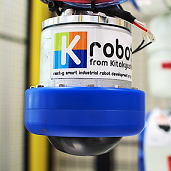
\includegraphics[scale=1,bb = 0 0 171 171]{fig/s_gripperp.png}
\end{figure}
\end{frame}

\end{document}
